\section{Algebraic FMM Variants}\label{chpt:2:sec:1}

In its original analytical form the applicability of the FMM is limited by the requirement for an explicit multipole and local expansions, as well as a restriction to matrix vector products. Subsequent decades saw the development of `algebraic' analogues to the original algorithm. These methods are similarly based on a hierarchical partitioning, whether that be of the point data using a recursive tree as with the original FMM \cite{Ying:2004:JCP,fong2009black}, or by operating on the matrix implied by the FMM's algorithmic structure directly \cite{hackbusch1999sparse,borm2003introduction,chandrasekaran2007fast}. The latter methods are collectively known as $\mathcal{H}$-matrix methods. Representing the FMM operation in this way has allowed extension of the FMM to other matrix computations, such as matrix-matrix products, as well as approximations of its inverse \cite{ambikasaran2014inverse}. Notably, many of these methods don't necessarily rely on explicit multipole/local expansions for approximating fields as in the original FMM in the previous section. Examples such as the `kernel independent FMM' (kiFMM) of Ying and co-authors instead relies on the method of fundamental solutions to approximate the fields and requires only evaluating kernel values, and is applicable to a wide range of kernels from second-order linear non-oscillatory elliptic PDEs with constant coefficients such as the Laplace equation. This approach relies on some analytic considerations, however methods also exist which are interpolatory - such as the `black box FMM' (bbFMM) of Fong and Darve \cite{fong2009black}, which similarly only relies on kernel evaluations and a Chebyshev scheme to approximate fields.

In our software we choose to implement the kiFMM of Ying and coauthors, which we explain in detail below adapting the discussion from Section 3 of \cite{Ying:2004:JCP}. This method shares advantages with other algebraic FMM methods, of generality to a large class of problems, as well as opportunities to optimise computer implementations we explore in Section \ref{chpt:2:sec:1}. This approach relies on a spatial discretisation of the problem domain via an quad/octree as in the original FMM, as well as the method of fundamental solutions (MFS) for approximating the fields from point charges/masses. This method has been demonstrated to scale well on shared \cite{wang2021exafmm} as well as distributed memory \cite{malhotra2015pvfmm} systems, achieve similar accuracy to the analytical variant, with relatively low pre-computation required. The underlying data structure of the quad/octree has been a significant area of research and development, with established high-performance methods for their construction in shared/distributed memory environments \cite{sundar2008bottom,sundar2013hyksort,BursteddeWilcoxGhattas11}.

Consider the kernels for second-order constant coefficient non-oscillatory PDEs, such as that of the Laplace equation in (\ref{eq:chpt:2:sec:0:laplace_kernel}). Such kernels satisfy the underlying PDE everywhere except the singularity location, and are smooth away from this singularity. These problems admit a unique solution for interior/exterior Dirichlet boundary value problems (see Appendix \ref{app:laplace_bvp} for a demonstration of this for the Laplace equation). The authors of \cite{Ying:2004:JCP} rely on the smoothness and uniqueness of the Dirichlet boundary value problems as basic properties to develop their FMM formulation. The problem setting as before is the calculation of (\ref{eq:chpt:2:sec:0:fmm_problem}) for the Laplace kernel, for a set of $N$ point sources $y_i$, $i = 1...N$, which we will associated with $N$ source densities $q_i$, an target locations $y_j$, $j=1...M$. As before, the source and target locations may coincide. We use an index set $I^B_s$ and $I^B_t$ to identify the sources and targets we are considering in a particular interaction. We assume that our problem is in $\mathbb{R}^3$, however the exposition is essentially the same as in $\mathbb{R}^2$.

Assuming that we have constructed our hierarchical tree partitioning, which may be adaptive, the first step is to approximate the fields due to particles contained in each leaf box. We specify more concretely that for a given box, $B$, its `near field range', $\mathcal{N}^B$, is the set of 27 boxes at the same level of a tree which are adjacent to it, i.e. they share a corner, face or edge as well as $B$ itself. Its `far field range', $\mathcal{F}^B$, is simply the boxes which are the complement of this.

We approximate the potential in $\mathcal{F}^B$ from the source densities $\{ q_i : i \in B \}$ in $B$ using the potential from an \textit{equivalent density distribution}, $q^{B, u}$, supported at prescribed locations $y^{B, u}$ (see the left box in Figure \ref{fig:chpt:2:sec:1:multipole_local}). Where $q^{B, u}$ is called the \textit{upward equivalent density} and $y^{B, u}$ is called the \textit{upward equivalent surface}. This amounts to representing the potential with a `single layer' potential \cite{Kress2014},

\begin{flalign}\label{eq:chpt:2:sec:1:single_layer_potential}
    \phi(x) &:= \int_{y \in y^{B, u}} q^{B, u}(y)K(x, y) ds(y), \> \> x \in \mathbb{R}^3 \setminus y^{B, u}
\end{flalign}

To guarantee the smoothness of the potential produced by $q^{B, u}$ in the far-field, its support $y^{B,u}$ must not overlap with $\mathcal{F}^B$ due to the singularities in this integral from the kernel function when evaluated on the equivalent surface. Secondly, we note that the equivalent surface must enclose $B$ from the definition of the single layer potential \cite{Kress2014}. We see that the equivalent surface must be placed in between the box and the boundary of $\mathcal{F}^B$.

The potential induced by our equivalent densities and upward equivalent surface satisfies the Laplace equation. Therefore, due to the uniqueness of the exterior Dirichlet boundary value problem for this kernel (as well of kernels of a similar type), we reason that the potential calculated using (\ref{eq:chpt:2:sec:0:fmm_problem}) directly from the source particles must be equivalent to that calculated using (\ref{eq:chpt:2:sec:1:single_layer_potential}) in $\mathcal{F}^B$, or anywhere between $y^{B, u}$ and $\mathcal{F}^B$. Thus we place an intermediate surface called the \textit{upward check surface} between $\mathcal{F}^B$ and $y^{B, u}$, denoting it with $x^{B, u}$. The potential computed at this surface is called the \textit{upward check potential}, which we denote by $\phi^{B, u}$.

We write this as,

\begin{flalign}\label{eq:chpt:2:sec:1:multipole_appx}
    \int_{y^{B, u}} K(x, y) q^{B, u} dy = \sum_{i \in I^B_s} K(x, y_i)q_i = \phi^{B, u}\> \>, \text{for any } x \in x^{B, u}
\end{flalign}

Solving for the equivalent densities is an equivalent method of approximating the far-field potential induced by the points in $B$. We identify this with a \textit{multipole expansion}. Now considering source densities which are not contained in a box $B$ (see right box of Figure \ref{fig:chpt:2:sec:1:multipole_local}) but in its $\mathcal{F}^B$, we can construct an equivalence for local expansions using a similar approach. To ensure the existence of the \textit{downward equivalent densities} $q^{B, d}$, the \textit{downward equivalent surface}, $y^{B, d}$, must be located between $B$ and $\mathcal{F}^B$ and the potentials generated by the source points are matched to those generated by the equivalent points on a \textit{downward check surface}, $x^{B, d}$ that encloses the box and is itself enclosed by $y^{B, d}$ in order to calculate a \textit{downward check potential} $\phi^{B, d}$.

\begin{flalign}\label{eq:chpt:2:sec:1:local_appx}
    \int_{y^{B, d}} K(x, y) q^{B, d} dy = \sum_{i \in I^{\mathcal{F}^B}_s} K(x, y_i)q_i = \phi^{B, d} \> \> \text{for any } x \in x^{B, d}
\end{flalign}

In $\mathbb{R}^3$ the authors chose to represent the equivalent and check surfaces as cubes, with the equivalent/check points arranged regularly over the surfaces. We choose the same as it leads to implementation benefits when designing the field translation operators (see Section \ref{chpt:1:sec:2} for how we take advantage of this).

\begin{figure}
    \centering
    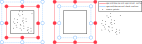
\includegraphics[width=\textwidth]{ch_2/p2m.pdf}
    \caption{ We illustrate the equivalent/check surfaces and associated boxes in $\mathbb{R}^3$, where we show a corresponding cross section. In the first figure, we illustrate the situation in the `P2M' operation, where we are trying to construct an approximation to the potential generated by points in a box by matching it to that generated by a set of equivalent density points placed on a fictitious surface enclosing it. In the second figure we illustrate the `P2L' operation, where we are now trying to construct an approximation to the  potential generated by points in a box's far-field within the box.}
    \label{fig:chpt:2:sec:1:multipole_local}
\end{figure}

Equations (\ref{eq:chpt:2:sec:1:multipole_appx}) and (\ref{eq:chpt:2:sec:1:local_appx}) are examples of \textit{Fredholm integral equations of the first kind}, the inversion of which is ill-posed. To solve these equations, we must first discretise, for which we made use of the \textit{Method of Fundamental Solutions} (MFS), a technique whereby the potential is approximated by a linear combination of kernel function evaluations at a set of discrete points with associated densities,

\begin{flalign}\label{eq:chpt:2:sec:1:mfs}
    \phi(x) \approx \phi^N(x) = \sum_{y_i \in y^{B, u}} K(x, y_i) q_i
\end{flalign}

Where $N$ denotes the number of equivalent points of density are placed on the equivalent surface. To see how this approximates the single-layer operator we used above to calculate the potential we simply replace the continuous density functions in (\ref{eq:chpt:2:sec:1:single_layer_potential}) with $\sum_{j=1}^N q_i \delta(y-y_j)$, recovering (\ref{eq:chpt:2:sec:1:mfs}). Writing (\ref{eq:chpt:2:sec:1:multipole_appx}) or (\ref{eq:chpt:2:sec:1:local_appx}) in matrix form reflecting the discretisation via MFS,

\begin{flalign}
    K q = \phi
\end{flalign}

We can solve the problem with Tikhonov regularisation,

\begin{flalign}
    q = (\alpha I + K^* K)^{-1}K^*\phi
\end{flalign}

which converts it into a \textit{Fredholm integral equation of the second kind} which are well-posed. The regularisation parameter $\alpha$ is found empirically. Computing (\ref{eq:chpt:2:sec:1:multipole_appx}) is equivalent to the $T^{P2M}$ operator described in the previous section for the analytical FMM, (\ref{eq:chpt:2:sec:1:local_appx}) is equivalent to an $T^{P2L}$ operator which was not explicitly described. As before, these operators take a set of charges, and create expansions that allow us to evaluate their potential in the far-field, however the method of creating the expansions is clearly significantly different. The most notable change being that our above formulation \textit{does not require explicit analytical expansions of the kernel function}, only making use of kernel evaluations.

To complete the kiFMM we need analogues to the field translation operators, $T^{M2L}$, $T^{M2M}$, $T^{L2L}$. We illustrate the required surfaces for each of these operators in Figure \ref{fig:chpt:2:sec:1:translations}. For $T^{M2M}$ we must translate the upward equivalent density of $A$ to the centre of its parent box $B$, solving the following equation for $q^{B, u}$,

\begin{flalign}
    \label{eq:chpt:2:sec:1:m2m}
    \int_{y^{B, u}} K(x, y)\phi^{B, u}(y)dy = \int_{y^{A, u}}K(x, y)\phi^{A, u}(y) dy, \> \> \text{for all } x \in x^{B, u}
\end{flalign}

As before, $y^{A, u}$ must enclose the child box $A$. During the downward pass, we must evaluate the downward equivalent density, corresponding to a local expansion, from the multipole expansions of non-adjacent boxes in $B$'s parent neighbour's children. We similarly write down for $T^{M2L}$,

\begin{flalign}
    \label{eq:chpt:2:sec:1:m2l}
    \int_{y^{B, d}} K(x, y)\phi^{B, d}(y)dy = \int_{y^{A, u}}K(x, y)\phi^{A, u}(y) dy, \> \> \text{for all } x \in x^{B, d}
\end{flalign}

Finally, the local expansions of each box $B$ must be translated to the centre of each of its children $A$,

\begin{flalign}
    \label{eq:chpt:2:sec:1:l2l}
    \int_{y^{B, d}} K(x, y)\phi^{B, d}(y)dy = \int_{y^{A, d}}K(x, y)\phi^{A, d}(y) dy, \> \> \text{for all } x \in x^{B, d}
\end{flalign}

For each of these translation operators we use the discretisation based on MFS discussed above, and solve using Tikhonov regularisation. For the  $T^{L2P}$, $P2P$ and $T^{M2P}$ operators we simply use direct kernel evaluations at the target points with respect to the equivalent densities represented by the multipole or local expansion coefficients or the true densities at the source points.

\begin{figure}
    \centering
    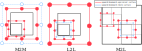
\includegraphics[width=\textwidth]{ch_2/translations.pdf}
    \caption{ As in Figure \ref{fig:chpt:2:sec:1:multipole_local}, we illustrate the translations as cross sections of the surfaces, which are cubes in $\mathbb{R}^3$.}
    \label{fig:chpt:2:sec:1:translations}
\end{figure}

